\documentclass{article}

\usepackage{polski}
\usepackage{amsmath}
\usepackage{graphicx}
\usepackage{float}
\usepackage{subfig}
\usepackage{multirow}

\title{Interpolacja według metod Lagrange'a oraz Newtona}
\author{\textbf{Łukasz Wala}\\
    \textit{AGH, Wydział Informatyki, Elektroniki i Telekomunikacji} \\
    \textit{Metody Obliczeniowe w Nauce i Technice 2021/2022}}
\date{Kraków, \today}

\begin{document}
\maketitle

\section{Opis problemu}
Główną ideą zadania jest zbadanie zachowania wielomianów interpolacyjnych dla poniższej funkcji, dla zagadnienia Lagrange'a, skonstruowanych dwoma metodami: Newtona oraz 
Lagrange'a oraz korzystając z różnego rozmieszczenia węzłów: równomiernie oddalonych oraz według pierwiastków wielomianu Czebyszewa.

Badana funkcja:
\[f(x)=x^2-m\cdot\cos\left(\frac{\pi x}{k}\right)\]
Gdzie $k=\frac{1}{2}$, $m=4$ oraz $x\in [-6,6]$.


\section{Opracowanie}
Pierwszym krokiem będzie skonstuowanie wielomianów dla różnych liczb węzłow oraz narysowanie wykresów. 
Do tego użyty zostanie załączony program w języku Python. 

\begin{figure}[H]
    \centering
    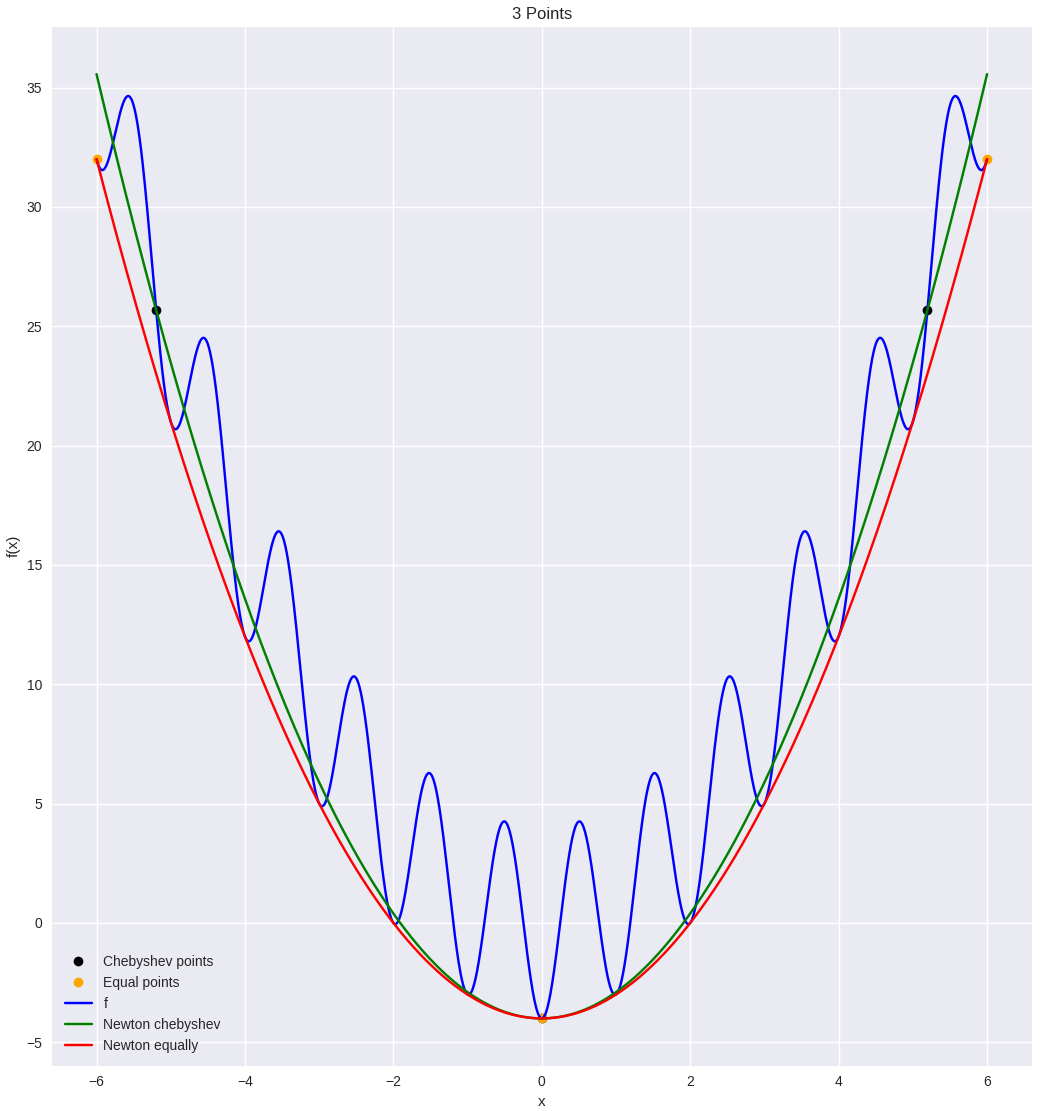
\includegraphics[width=0.6\textwidth]{img/newt_3.png}
    \caption{Metoda Newtona dla 3 punktów}
\end{figure}

Dla 3 węzłów wykres wielomianu nie przypomina zbytnio wykresu funkcji $f$, co nie powinno dziwić. Podobnie w przypadku metody Lagrange'a:

\begin{figure}[H]
    \centering
    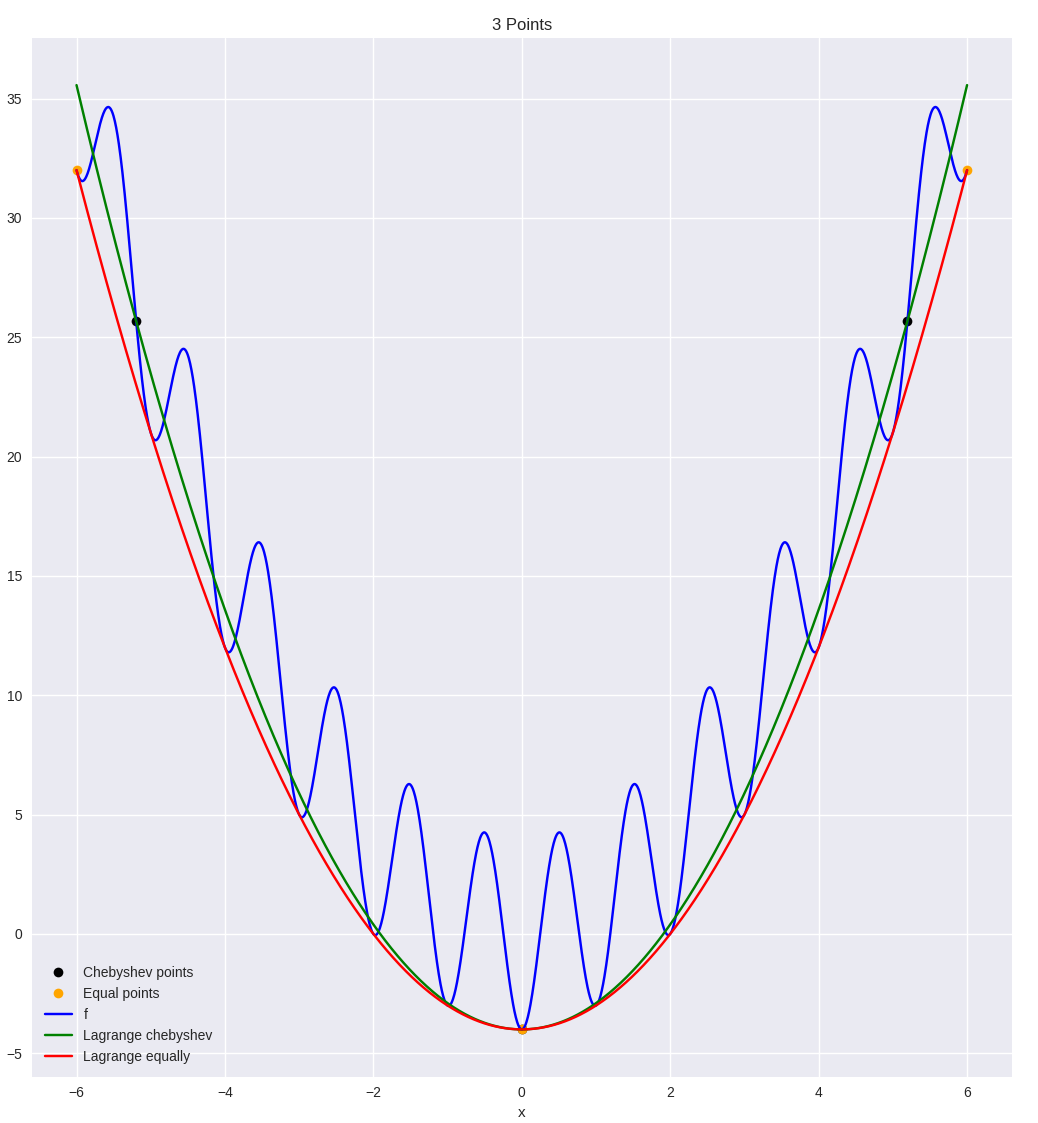
\includegraphics[width=0.6\textwidth]{img/lagr_3.png}
    \caption{Metoda Lagrange'a dla 3 punktów}
\end{figure}

Wraz z zwiększaniem liczby węzłów wykres wielomianu coraz bardziej zbliża się do wykresu funkcji $f$, 
poniżej przykład dla 15 węzłów, dla obu metod rozmieszczenia węzłów wyniki są wizualnie podobne.

\begin{figure}[H]
    \centering
    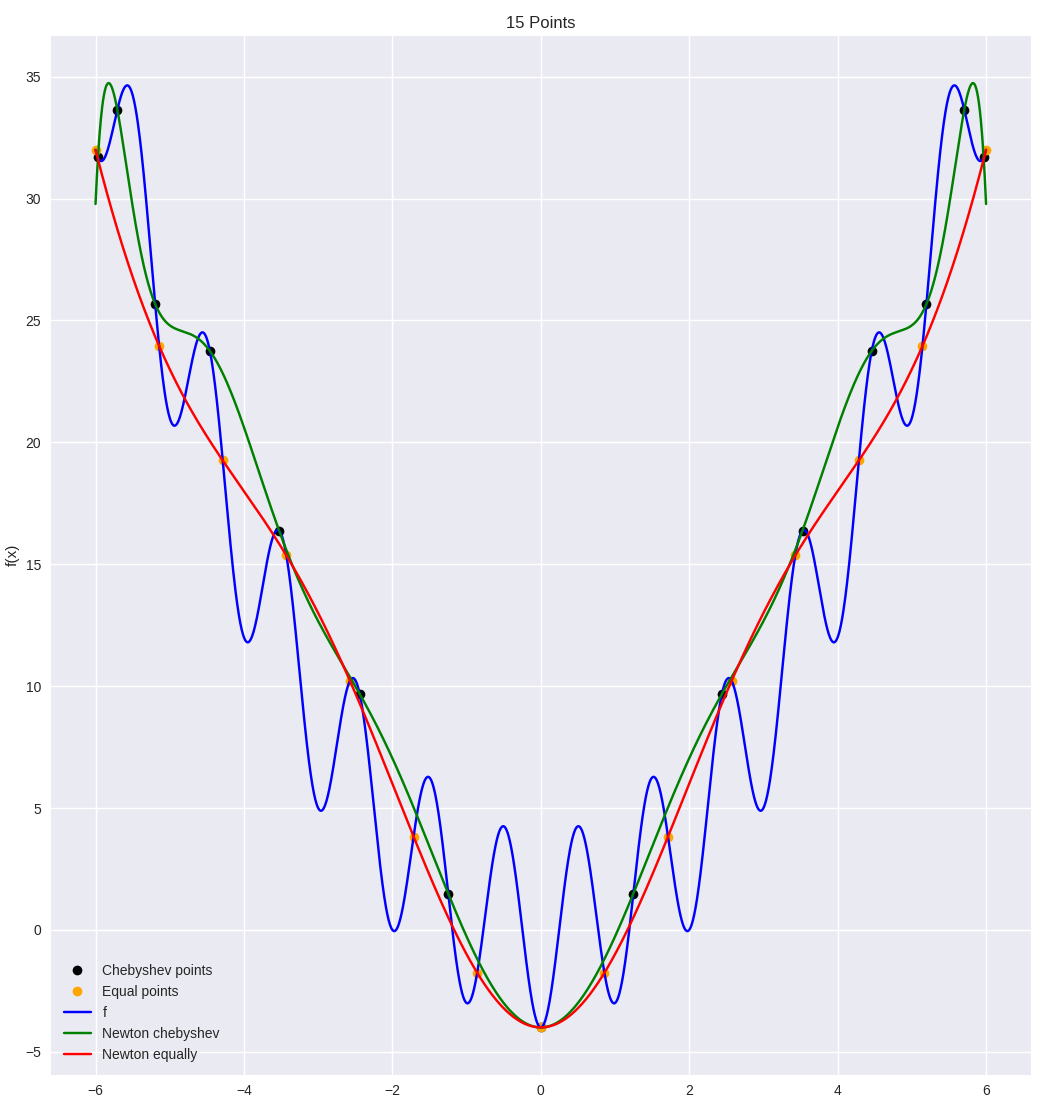
\includegraphics[width=0.9\textwidth]{img/newt_15.png}
    \caption{Metoda Newtona dla 15 punktów}
\end{figure}

Jednak dla ok. 17-18 węzłów w przypadku równomiernego rozmieszczenia węzłów, na krańcach przedziału zaczyna być widoczny efekt 
Rungego. Wraz z dalszym zwiększaniem liczby węzłów dla rozłożenia równomiernego efekt pogłębia się, a co za tym idzie,
jakość interpolacji spada. Występowanie efektu Rungego nie jest zależne od metody interpolacji, natomiast nie występuje w przypadku węzłów 
Czebyszewa, które są gęściej upakowane na krańcach przedziału.

\begin{figure}[H]
    \centering
    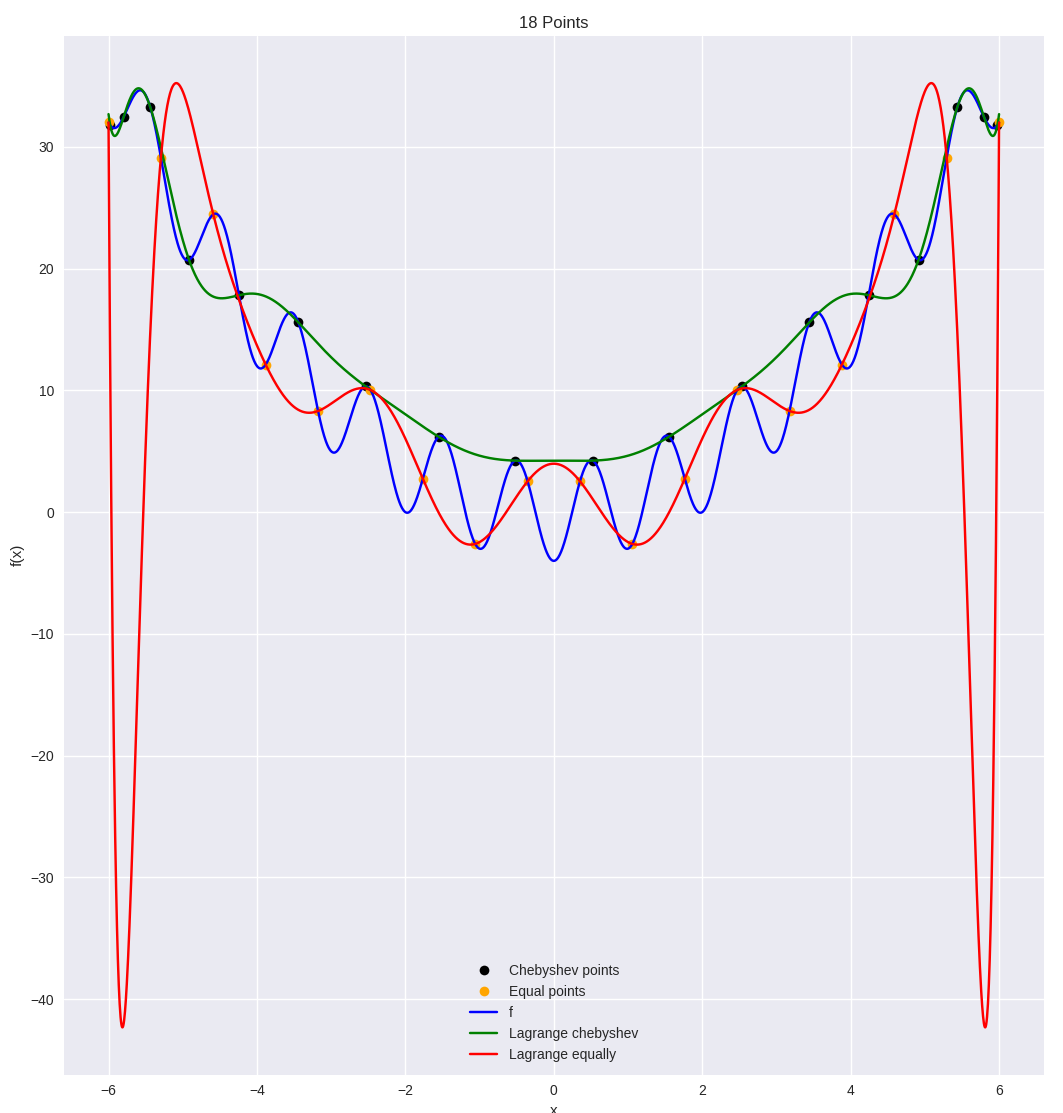
\includegraphics[width=\textwidth]{img/lagr_18.png}
    \caption{Metoda Lagrange'a dla 18 punktów}
\end{figure}

Podobieństwo wielomianu do funkcji $f$ dla węzłów Czebyszewa rośnie dla obu metod aż do liczby 38 węzłów, gdzie następuje degradacja
jakości wielomianu oraz pojawiają się błędy (wielomian nie zawiera punktów w węzłach) dla metody Newtona przy krańcach przedziału. Problem 
najprawdopodobniej wynika z błędów obliczeń związanymi z ograniczeniami precyzji floata. Na poniższym wykresie efekt ten zaczyna być zauważalny dla lewego krańca
przedziału dla węzłow Czebyszewa (oraz bardzo ewidentny efekt Rungego dla równomiernie rozmieszczonych węzłów).

\begin{figure}[H]
    \centering
    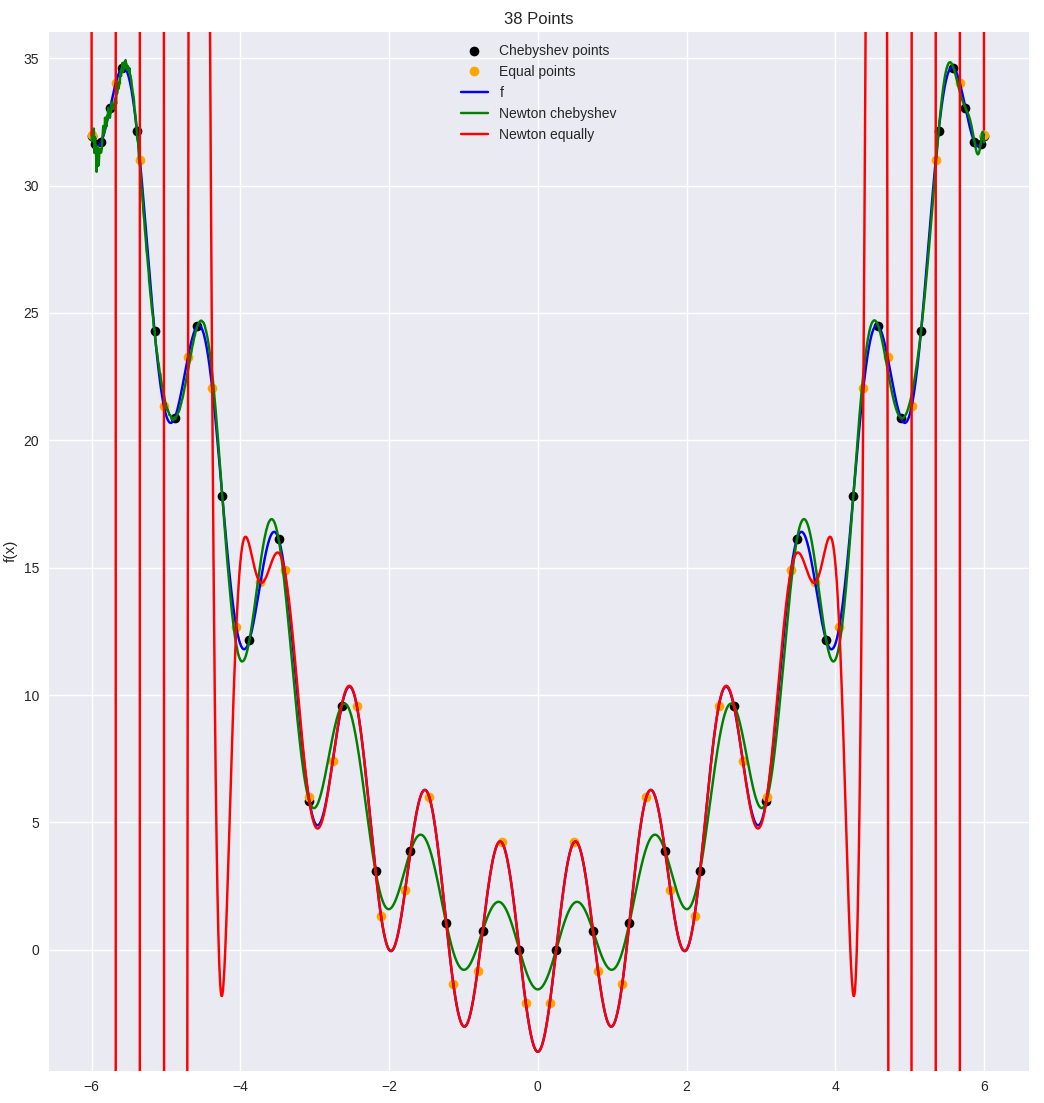
\includegraphics[width=\textwidth]{img/newt_38.png}
    \caption{Metoda Newtona dla 38 punktów}
\end{figure}

Dla 50 węzłów, będącą największą zbadaną wartością, metoda Lagrange'a dla węzłów Czebyszewa bardzo dokładnie w przybliża
funkcję $f$. Pozostałe metody, ze względu na efekt Rungego lub problem opisany na stronie 4, nie są w stanie przybilżyć funkcji.

\begin{figure}[H]
    \centering
    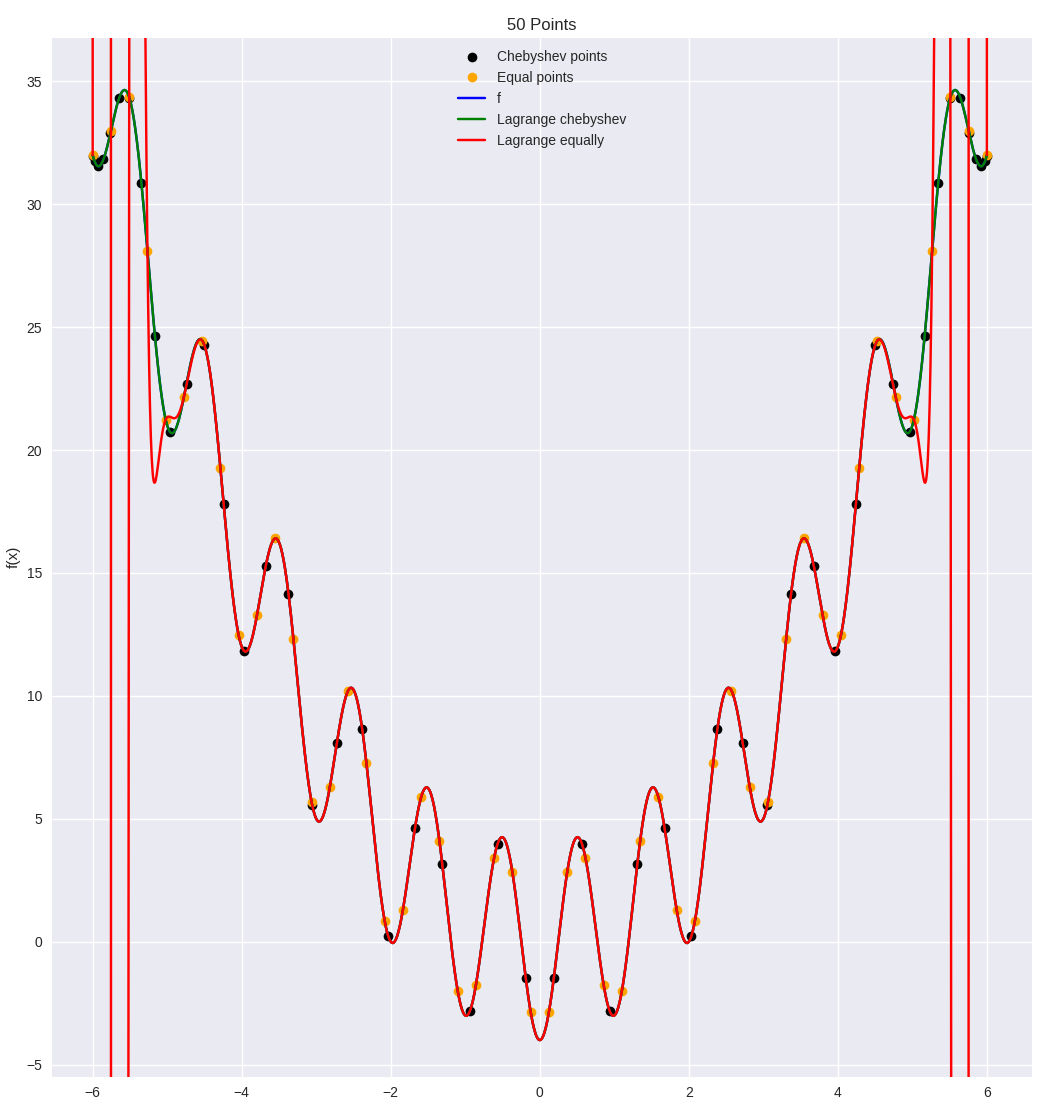
\includegraphics[width=0.6\textwidth]{img/lagr_50.png}
    \caption{Metoda Lagrange'a dla 50 punktów}
\end{figure}

\begin{figure}[H]
    \centering
    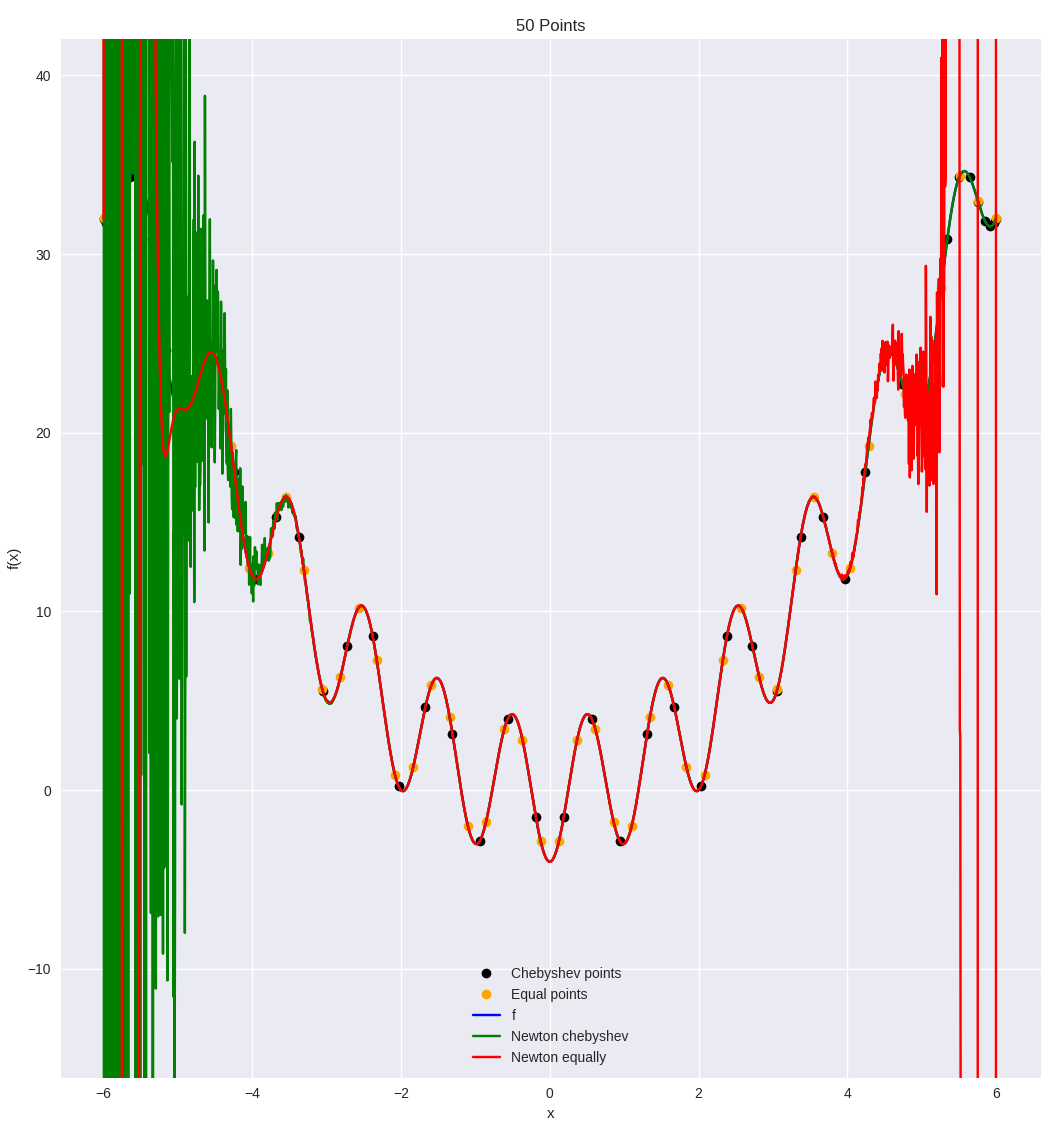
\includegraphics[width=0.6\textwidth]{img/newt_50.png}
    \caption{Metoda Newtona dla 50 punktów}
\end{figure}

Kolejnym krokiem będzie policzenie dokładności przybliżenia. Miarami dokładności będą: średnia kwadratów odległości wartości odległości oraz największa różnica wartości odległości 
funkcji $f$ oraz wielomianu interpolacyjnego dla 1000 równomiernie rozmieszczonych punktów w zakresie $[-6,6]$. Poniższe tabele
zawierają dokładności od 3 do 49, mierząc co drugą liczbę węzłów.

\begin{table}[H]
    \centering
    \begin{tabular}{|l|ll|ll|}
    \hline
    \multicolumn{1}{|c|}{\multirow{2}{*}{\begin{tabular}[c]{@{}c@{}}Liczba \\ węzłów\end{tabular}}} &
      \multicolumn{2}{c|}{Newton} &
      \multicolumn{2}{c|}{Lagrange} \\ \cline{2-5} 
    \multicolumn{1}{|c|}{} &
      \multicolumn{1}{c|}{Czebyszew} &
      \multicolumn{1}{c|}{rów. odd.} &
      \multicolumn{1}{c|}{Czebyszew} &
      \multicolumn{1}{c|}{rów. odd.} \\ \hline
    3 & \multicolumn{1}{l|}{17.0733} & 23.98  & \multicolumn{1}{l|}{17.0733} & 23.98 \\ \hline
    5 & \multicolumn{1}{l|}{18.8049}  & 23.98  & \multicolumn{1}{l|}{18.8049}  &  23.98 \\ \hline
    7 & \multicolumn{1}{l|}{16.5071}  & 23.98  & \multicolumn{1}{l|}{16.5071}  &  23.98 \\ \hline
    9 & \multicolumn{1}{l|}{17.7717}  & 225.44  & \multicolumn{1}{l|}{17.7717}  &  225.44 \\ \hline
    11& \multicolumn{1}{l|}{15.0579}  & 16.10  & \multicolumn{1}{l|}{15.0579}  &  16.10 \\ \hline
    13& \multicolumn{1}{l|}{16.4392}  & 23.98  & \multicolumn{1}{l|}{16.4392}  &  23.98 \\ \hline
    15& \multicolumn{1}{l|}{16.6307}  & 15.98  & \multicolumn{1}{l|}{16.6307}  &  15.98 \\ \hline
    17& \multicolumn{1}{l|}{14.8798}  & 14.81  & \multicolumn{1}{l|}{14.8798}  &  14.81 \\ \hline
    19& \multicolumn{1}{l|}{15.7795}  & 18855.10  & \multicolumn{1}{l|}{15.7795}  &  18855.10 \\ \hline
    21& \multicolumn{1}{l|}{13.1300}  & 7825523.53  & \multicolumn{1}{l|}{13.1300}  &  7825523.53 \\ \hline
    23& \multicolumn{1}{l|}{12.6171}  & 513891521.49  & \multicolumn{1}{l|}{12.6171}  &  513891521.49 \\ \hline
    25& \multicolumn{1}{l|}{11.3945}  & 9781348058  & \multicolumn{1}{l|}{11.3945}  & 9781348058 \\ \hline
    27& \multicolumn{1}{l|}{11.2069}  & 76060415066  & \multicolumn{1}{l|}{11.2069}  &  76060415071 \\ \hline
    29& \multicolumn{1}{l|}{9.5034}  & 297334254455  & \multicolumn{1}{l|}{9.5034}  &  297334254506 \\ \hline
    31& \multicolumn{1}{l|}{8.8444}  & 667288797764  & \multicolumn{1}{l|}{8.8444}  & 667288797931  \\ \hline
    33& \multicolumn{1}{l|}{7.8320}  & 940961326952 & \multicolumn{1}{l|}{7.8321}  &  940961329998 \\ \hline
    35& \multicolumn{1}{l|}{4.1558}  &  889414296556 & \multicolumn{1}{l|}{4.1555}  &  889414307658 \\ \hline
    37& \multicolumn{1}{l|}{1.3042}  & 591429140136  & \multicolumn{1}{l|}{1.2971}  &  591429134229 \\ \hline
    39& \multicolumn{1}{l|}{0.2676}  &  287215295287 & \multicolumn{1}{l|}{0.2574}  &  287215301381 \\ \hline
    42& \multicolumn{1}{l|}{0.4426}  & 104940098714  & \multicolumn{1}{l|}{0.03472}  &  104940003048 \\ \hline
    43& \multicolumn{1}{l|}{1.0863}  &  29554893468 & \multicolumn{1}{l|}{0.003348}  & 29554762315  \\ \hline
    45& \multicolumn{1}{l|}{10.7866}  & 6546668681  & \multicolumn{1}{l|}{0.00023972}  &  6546450581 \\ \hline
    47& \multicolumn{1}{l|}{734.1665}  & 1160128264  & \multicolumn{1}{l|}{0.00001312}  &  1159986609 \\ \hline
    49& \multicolumn{1}{l|}{396.5238}  & 166848078  & \multicolumn{1}{l|}{0.00000056}  &  166833341 \\ \hline
    \end{tabular}
    \caption{Średnia kwadratów różnic funkcji $f$ oraz wielomianów}
\end{table}

Wnioski uzyskane podczas analizy wykresów zgadzają się z zawartością tabeli: dla liczb węzłów mniejszych niż 18 wyniki są niemal identyczne
niezależnie od metody lub rozmieszczenia węzłów. Równomiernie rozmieszczone punkty skutkują stratą dokładności przy liczbie 
węzłów większej niż ok. 18 (efekt Rungego), natomiast dokładność metody Newtona zaczyna maleć
po przekroczeniu liczby ok. 40 węzłów (problem opisany na 4 stronie). Najdokładniejsza okazuje się metoda Lagrange'a dla węzłów
Czebyszewa, której dokładność rośnie dla całej puli badanych liczb węzłów. Liczba węzłów, dal której uzyskano największą
dokładność z użyciem załączonego programu (ze względu na długi czas działania) to 79, przy czym można przypuszczać, że dokładność nadal rośnie dla większych liczb.

Poniższa tabela maksiumów wartości odległości w punktach dla wielomianu oraz funkcji $f$ utwierdza w dotychczasowych wnioskach.

\begin{table}[H]
    \centering
    \begin{tabular}{|l|ll|ll|}
    \hline
    \multicolumn{1}{|c|}{\multirow{2}{*}{\begin{tabular}[c]{@{}c@{}}Liczba \\ węzłów\end{tabular}}} &
        \multicolumn{2}{c|}{Newton} &
        \multicolumn{2}{c|}{Lagrange} \\ \cline{2-5} 
    \multicolumn{1}{|c|}{} &
        \multicolumn{1}{c|}{Czebyszew} &
        \multicolumn{1}{c|}{rów. odd.} &
        \multicolumn{1}{c|}{Czebyszew} &
        \multicolumn{1}{c|}{rów. odd.} \\ \hline
    3 & \multicolumn{1}{l|}{7.9752} & 7.9998  & \multicolumn{1}{l|}{7.9752} &  7.9998\\ \hline
    5 & \multicolumn{1}{l|}{8.8575}  &  7.9998 & \multicolumn{1}{l|}{8.8575}  &  7.9998 \\ \hline
    7 & \multicolumn{1}{l|}{8.1337}  & 7.9998  & \multicolumn{1}{l|}{8.1337}  &  7.9998 \\ \hline
    9 & \multicolumn{1}{l|}{7.9917}  &  37.2665 & \multicolumn{1}{l|}{7.9917}  &  37.2665 \\ \hline
    11& \multicolumn{1}{l|}{10.0078}  & 7.9964 & \multicolumn{1}{l|}{10.007}  & 7.9964  \\ \hline
    13& \multicolumn{1}{l|}{8.0206}  &  7.9998 & \multicolumn{1}{l|}{8.0206}  &  7.9998 \\ \hline
    15& \multicolumn{1}{l|}{8.6225}  & 7.9992  & \multicolumn{1}{l|}{8.6225}  &  7.9992 \\ \hline
    17& \multicolumn{1}{l|}{7.8088}  &  6.2050 & \multicolumn{1}{l|}{7.8088}  &  6.2050 \\ \hline
    19& \multicolumn{1}{l|}{8.1167}  & 648.82  & \multicolumn{1}{l|}{8.1167}  &  648.829 \\ \hline
    21& \multicolumn{1}{l|}{8.6439}  &  14045.280 & \multicolumn{1}{l|}{8.6439}  &  14045.2 \\ \hline
    23& \multicolumn{1}{l|}{8.0000}  & 120159.07  & \multicolumn{1}{l|}{8.0000}  &  120159.0 \\ \hline
    25& \multicolumn{1}{l|}{8.3273}  & 551407.06  & \multicolumn{1}{l|}{8.3273}  & 551407.0 \\ \hline
    27& \multicolumn{1}{l|}{7.8523}  & 1611826  & \multicolumn{1}{l|}{7.8523}  &  1611826 \\ \hline
    29& \multicolumn{1}{l|}{8.2379}  &  3327716 & \multicolumn{1}{l|}{8.2379}  &  3327716 \\ \hline
    31& \multicolumn{1}{l|}{7.8731}  &  5187650 & \multicolumn{1}{l|}{7.8731}  & 5187650  \\ \hline
    33& \multicolumn{1}{l|}{6.1203}  & 6409255 & \multicolumn{1}{l|}{6.1203}  &  6409255 \\ \hline
    35& \multicolumn{1}{l|}{3.8940}  &  6437258 & \multicolumn{1}{l|}{3.8940}  &  6437258 \\ \hline
    37& \multicolumn{1}{l|}{2.0243}  &  5444504 & \multicolumn{1}{l|}{2.0243}  &  5444504 \\ \hline
    39& \multicolumn{1}{l|}{1.4708}  &  3909357 & \multicolumn{1}{l|}{0.8717}  & 3909357  \\ \hline
    42& \multicolumn{1}{l|}{9.8612}  & 2433404  & \multicolumn{1}{l|}{0.3185}  &  2433401 \\ \hline
    43& \multicolumn{1}{l|}{13.3245}  &  1331536 & \multicolumn{1}{l|}{0.09962}  & 1331533  \\ \hline
    45& \multicolumn{1}{l|}{42.691}  &  642940 & \multicolumn{1}{l|}{0.02706}  &  642916 \\ \hline
    47& \multicolumn{1}{l|}{333.59}  & 276428  & \multicolumn{1}{l|}{0.00645}  &  276373 \\ \hline
    49& \multicolumn{1}{l|}{266.21}  & 107818  & \multicolumn{1}{l|}{0.001365}  &  107818 \\ \hline
    \end{tabular}
    \caption{Maksimum wartości bezwględnej różnic funkcji $f$ oraz wielomianów}
\end{table}


\section{Wnioski}
Zarówno metoda Newtona jak i Lagrange'a pozwala na skuteczne przybliżanie funkcji z użyciem wielomianów interpolacyjnych przy zachowaniu 
pewnych warunków, np. używaniu węzłów Czebyszewa, żeby uniknąć efektu Rungego. Użycie tych metod może być przydatne, jeżeli funkcja przybliżana
jest skomplikowana i wygodniejsze jest używanie wielomianu interpolacyjnego lub gdy znane są tylko niektóre wartości funkcji.


\end{document}